\documentclass[12pt]{article}

\usepackage{graphicx}
\usepackage{pdfpages}
\usepackage{listings}
\usepackage{amsmath}
\usepackage{subcaption}
\usepackage{todonotes}

\renewcommand{\figurename}{Fig.}

\title{TTK4210 Advanced Control of Industrial Systems, Exercise 6}
\date{}
\author{Kristian Løvland}

\begin{document}
\maketitle
\tableofcontents

\newpage
\section{Abstract}
In this project, a model of a distillation column is used to design a controller for the composition of two product streams consisting of n-butane and iso-butane, respectively. \todo[inline]{Legg til resultater}

\newpage
\section{Introduction}
The stream of control engineers is flowing slower than before, but still steadily into lucrative jobs in the process industry. As a part of this, all children learn about hydrocarbon chains in middle school, and every cybernetics student at NTNU learns how to control plants that are common in the petroleum industry. This report is simply me doing my part.

A good introduction to the control problem we're faced with is given in the assignment text \todo{Legg til kilde}. A short summary of this follows here.

Our final goal is to have a control system giving two product flows out of the distillation column having the desired compositions $x_D^*$ and $x_B^*$. In practice, we control our compositions $x_D$ and $x_B$ indirectly through the temperatures in the locations of the product streams, denoted $T_D$ and $T_B$.

To achieve this, some more control is needed. The levels $M_D$ and in the top accumulator and $M_B$ in the destillation column needs to be controlled to stable setpoints. The same goes for distillation column pressure $p$.

To control these five variables, five degrees of freedom is needed. These are all flow rates, denoted $V_T$, $L$, $D$, $V$, $B$. Each of these is controlled more or less directly by a valve.

Independent control of all of the variables are used. Table \ref{tab:pairings} shows the pairing of manipulated and controlled variables. It is assumed that choosing godd setpoints for $T_D$ and $T_B$ gives satisfactory product quality. The control structure used here is called LV-control, after the manipulated variables used to (indirectly) control product quality.

\begin{table}[h]
\centering
\begin{tabular}{c|c}
Manipulated variable & Controlled variable \\ \hline
$V_T$ & $p$ \\
$D$ & $M_D$ \\
$B$ & $M_B$ \\
$L$ & $T_D$ \\
$V$ & $T_B$
\end{tabular}
\caption{Variable pairings}
\label{tab_pairings}
\end{table}

\subsection{A few words on scaling}
The scaling and units used in this report might seem a bit arbitrary. Despite how it might seem, I have tried to be consistent. For my own sake, all plots of variables are in engineering units, the same goes for all controller gains $K_p$. These have been converted to internally scaled gain when implementing the controllers in K-spice. Units (or the lack of them) for plots used in frequency analysis and loop-shaping are hopefully unambiguous.

\newpage
\section{Tuning secondary controllers}
The secondary controllers were tuned individually using the SIMC method for PI controllers. A step in process input with an amplitude small enough to not cause problems (usually meaning 50\% of maximum accepted input magnitude) in other parts of the system was used for all the secondary controllers, controlling the states $D$, $L$, $B$, $V$ and $p$.

In short, the SIMC tuning method can be summarized as follows (using notation from \cite{regtek}) \todo{Legg til kilde, regtekboka}

\begin{enumerate}
\item Fit the step response to a first order model. This means finding time delay $\tau$, slope $k' = \frac{dy/dt}{\Delta u}$ and time constant $T_1$ from the plot of the step response.
\item To achieve the desired time constant $T_L$, use the PI controller parameters $K_p = \frac{1}{k'} \frac{1}{\tau + T_L}$, $T_i = \min(T_1, 4(\tau + T_L))$.
\end{enumerate}

% Figurer, open-loop stegrespons
\begin{figure}
\centering
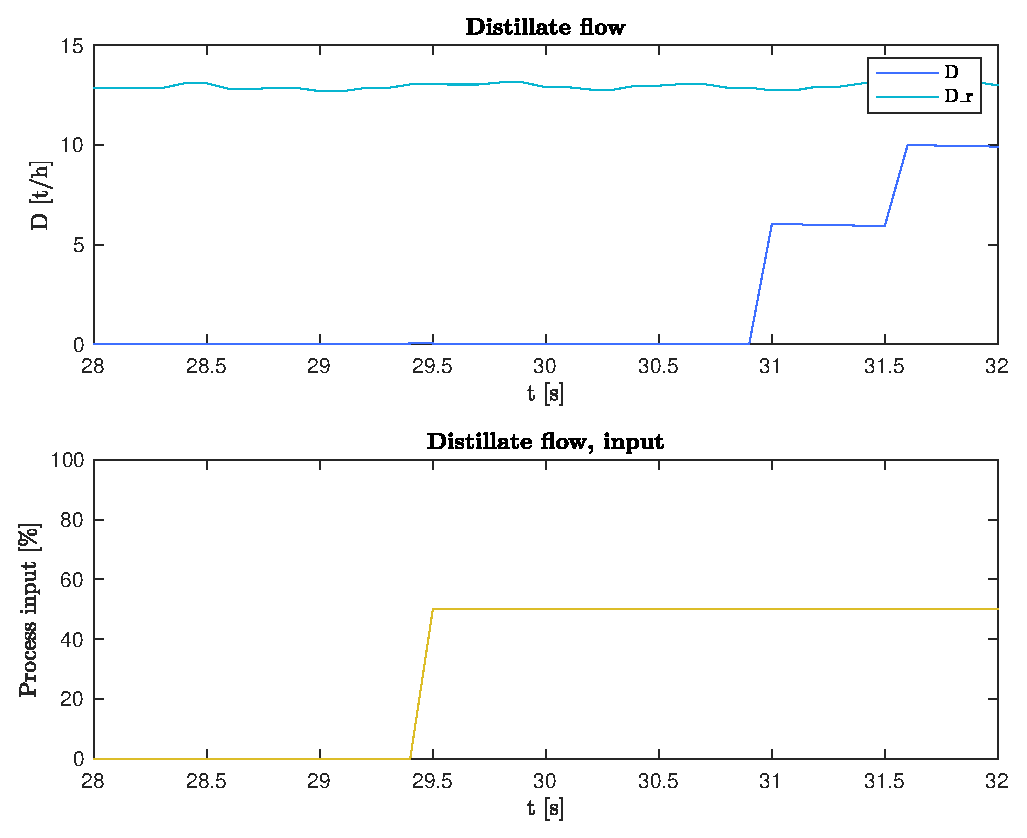
\includegraphics[width=0.8\textwidth]{../Systemanalyse/Log_Data_to_Matlab/Figurer/Stegeksperimenter/FC1005.eps}
\caption{Open-loop step response of $D$}
\label{fig:ol_step_FC1005}
\end{figure}

\begin{figure}
\centering
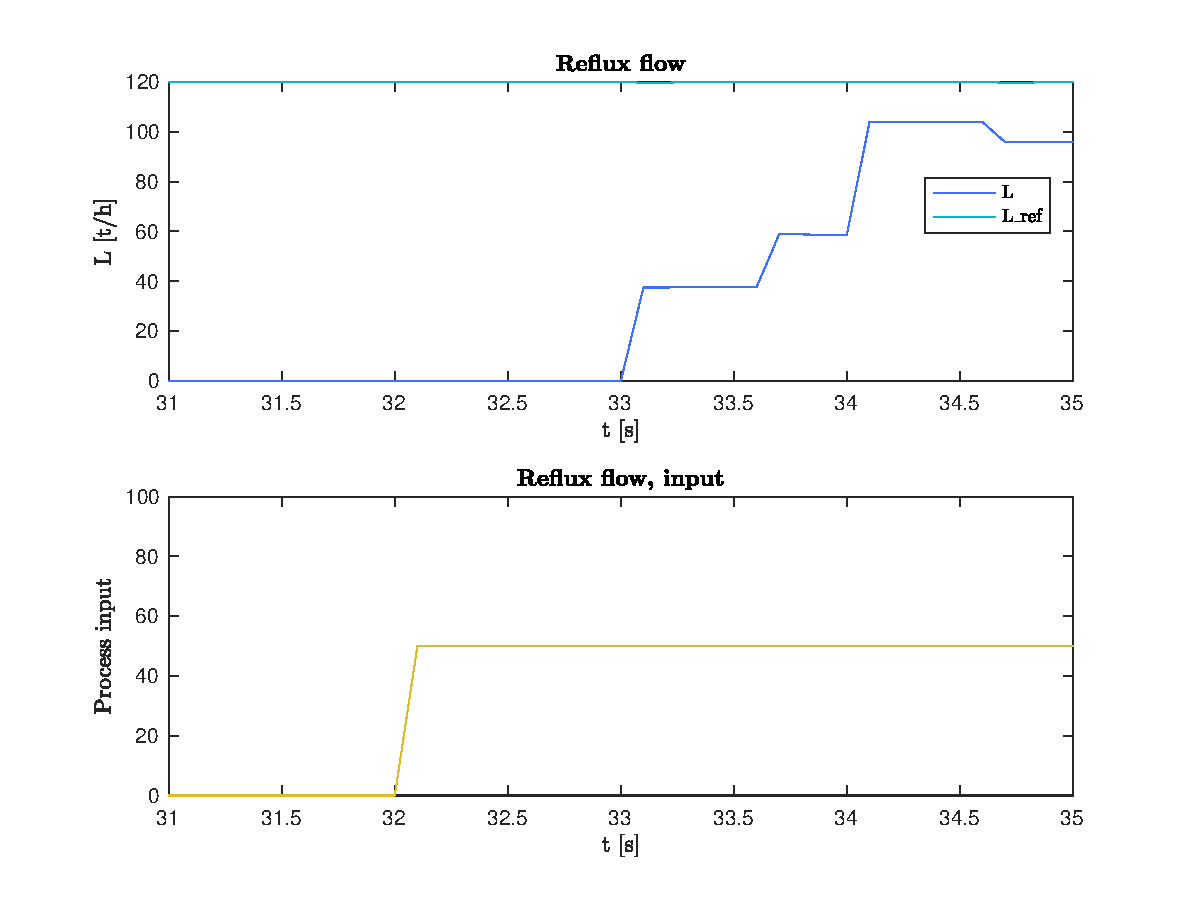
\includegraphics[width=0.8\textwidth]{../Systemanalyse/Log_Data_to_Matlab/Figurer/Stegeksperimenter/FC1015.eps}
\caption{Open-loop step response of $L$}
\label{fig:ol_step_FC1015}
\end{figure}

\begin{figure}
\centering
\includegraphics[width=0.8\textwidth]{../Systemanalyse/Log_Data_to_Matlab/Figurer/Stegeksperimenter/FC1019.eps}
\caption{Open-loop step response of $B$}
\label{fig:ol_step_FC1019}
\end{figure}

\begin{figure}
\centering
\includegraphics[width=0.8\textwidth]{../Systemanalyse/Log_Data_to_Matlab/Figurer/Stegeksperimenter/LC1028.eps}
\caption{Open-loop step response of heat exchanger area, related to $V$}
\label{fig:ol_step_LC1028}
\end{figure}

\begin{figure}
\centering
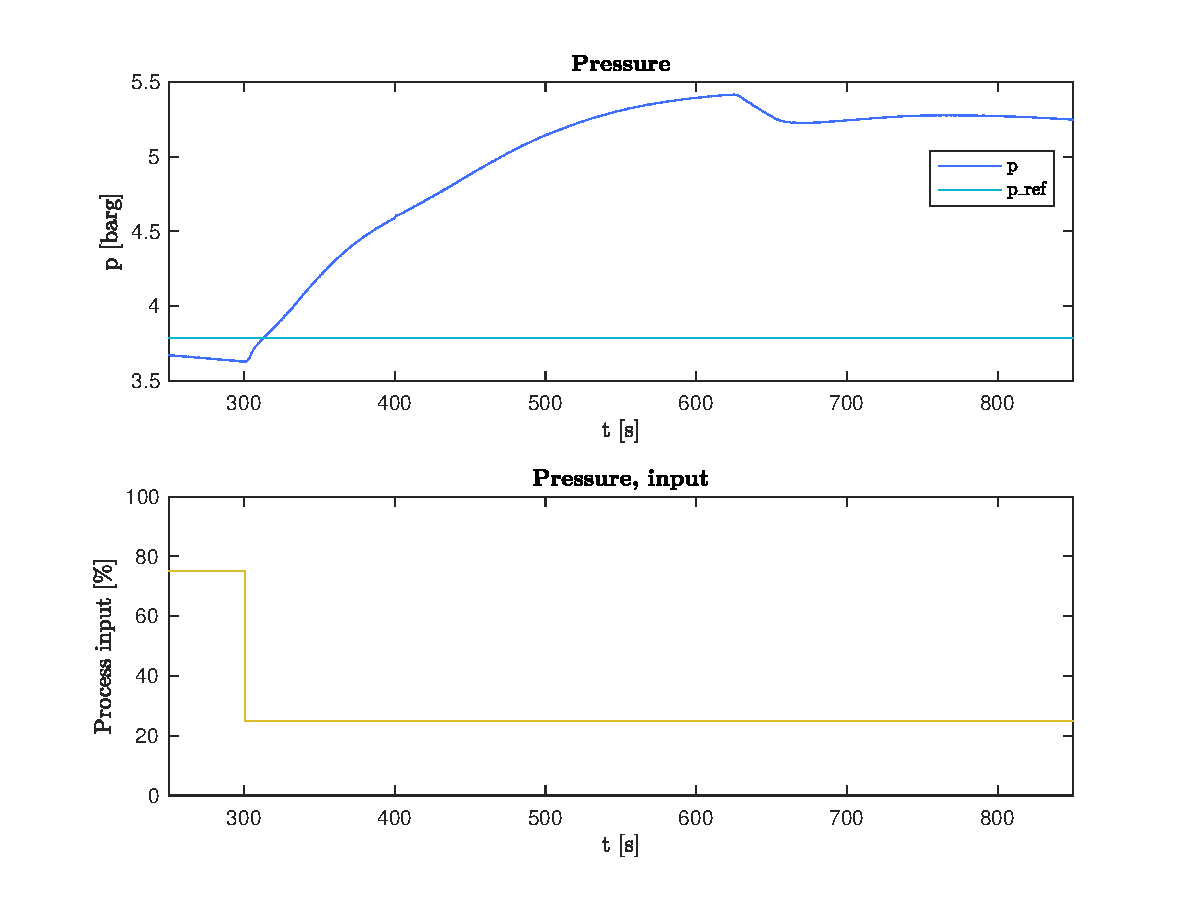
\includegraphics[width=0.8\textwidth]{../Systemanalyse/Log_Data_to_Matlab/Figurer/Stegeksperimenter/PC1024.eps}
\caption{Open-loop step response of $p$}
\label{fig:ol_step_PC1024}
\end{figure}

The data from these experiments can be seen in figures \ref{fig:ol_step_FC1005}, \ref{fig:ol_step_FC1015}, \ref{fig:ol_step_FC1019}, \ref{fig:ol_step_LC1028} and \ref{fig:ol_step_PC1024}. The reference signals should have been omitted from these plots since we are dealing with open loop systems, and can safely be ignored here.

The plots show that for the first three variables, the accuracies of the simulations are clearly not sufficient for fitting a first order model (they behave in a stepwise fashion). Inspecting the order of magnitude of the gains and time constants is, however, still useful. An attempt at making sense of these parameters is shown in table \ref{tab:inner_loop_step_responses}, together with the fitted values for $V$ and $p$.

Simple linear interpolation from initial to steady-state value was used for the three quick states, which gives conservative estimates of $k'$ and $T_1$. In the table, a desired time constant for the controlled system $T_L$ is shown in the rightmost column. For a quick response, choosing $T_L = 0,3\tau$ is suggested in \cite{balchen}. Some simple trial and error in K-spice showed that this lead to oscillation and unfortunate interaction between control loops, especially the controllers for $D$ and $L$. This is probably partly due to the underestimates of $k'$ and $T_1$ for these variables, since conservative estimates of these results in more aggressive controllers (to compensate for the slow system) when using the SIMC method.

Due to this unsatisfactory behaviour, $T_L = 2\tau$ was chosen for the three fastest control loops instead. The time delay was hard to make a meaningful reading of for the two other systems, so a somewhat arbitrary choice of $T_L = 10s$ was chosen for these systems (instead of using the $T_L = 2\tau$ rule). Like all the other parameters, these were not absolute choices, but a good starting point for further tuning.

After calculating the SIMC controller values, some qualitative tuning using K-spice simulations was, not surprisingly, needed. Here, the integral times (which could be read decently well from the open-loop step response plots) were kept fixed. The resulting one degree of freedom made tuning easier, and the results of this tuning is shown in table \ref{tab:inner_loop_PI_parameters}, together with the values from the SIMC method (which served as the starting point for this tuning). A column showing the scaled gain $G = K_p \frac{(y_{\max} - y_{\min})}{(u_{\max} - u_{\min})}$, which is the value implemented in K-spice, is also shown. The final controller gains are also given in this variable, since the parameters were changed directly in the K-spice panel. The two slowest control loops were showing slow responses, and the controller parameters were adjusted to be more aggressive. $T_i$ in the $p$ control loop was changed from 40s to 20s in the final tuning, and $T_i$ was chosen to be 10s in the $V$ control loop.


\begin{table}
\centering
\begin{tabular}{c | c | c | c | c | c || c}
& $\tau$ & $T_1$ & $\frac{dy}{dt}$ & $\Delta u$ & $k'$ & $T_L$ \\ \hline
$D$ & 1,0s & 0,4s & 14,3 & 50\% & 28,6 & 2s \\
$L$ & 1,0s & 1,0s & 47,5 & 50\% & 95,0 & 2s \\
$B$ & 1,0s & 0,6s & 10,0 & 50\% & 20,0 & 2s \\
$V$ & $\approx$ 0 & 400s & 0,028 & 20\% & 0,14 & 10s \\
$p$ & $\approx$ 0 & 200s & 0,088 & 50\% & 0,18 & 10s
\end{tabular}
\caption{Identified parameters for inner loop}
\label{tab:inner_loop_step_responses}
\end{table}


\begin{table}
\centering
\begin{tabular}{c | c | c | c | c}
& $K_p$ & $T_i$ & $G_{\textrm{SIMC}}$ & $G_{\textrm{final}}$ \\ \hline
$D$ & 0,0035 & 0,4s & 0,42 & 0,42\\
$L$ & 0,0018 & 1,0s & 0,22 & 0,22\\
$B$ & 0,0083 & 1,0s & 1,0 & 0,30 \\
$V$ & 0,71 & 10s & 86 & 200 \\
$p$ & 0,57 & 20s & 68 & 30
\end{tabular}
\caption{PI controller parameters for inner loop}
\label{tab:inner_loop_PI_parameters}
\end{table}

\todo{Legg til noe om at resten av systemet bare var i tilfeldige tilstander med tilfeldige regulatorer.}

\todo{Regn ut riktige verdier (det er feil i reg.parameterverditabellen), og avfei disse}

\newpage
\section{Level controllers}
\subsection{System identification}
\todo[inline]{Dette}
\subsection{Controller tuning}
\todo[inline]{Frekvensanalyse som rettferdiggjør initielle regulatorparametre}
The parameters are shown in table \ref{tab:DB_parameters}, together with the parameters gained from a second round of tuning using K-spice simulations.

\begin{table}[h]
\centering
\begin{tabular}{c | c | c | c | c}
 & $K_{p, \textrm{initial}}$ & $T_{i, \textrm{initial}}$ & $K_{p, \textrm{second}}$ & $T_{i, \textrm{second}}$\\ \hline
 $D$ & 830 & 1000s & & \\
 $B$ & 1000 & 1000s & &
\end{tabular}
\caption{Parameters for level controllers}
\end{table}

\newpage
\section{Composition controllers}
\subsection{System identification}
\todo[inline]{Dette}
\subsection{Controller tuning}
\todo[inline]{Dette}

\end{document}
